%\section{Solution design (i mangel af bedre navn}
%This section describes the design of the system as it is implemented. First, system architecture will be presented as to gain an overview of how the system works on a high level. Then the communication between modules will be discussed, following a description of data preprocessing and analysis. At last we discuss how the route planning module of the system works.
\section{System architecture}
The design in \figref{fig:systemoverview} shows the overview of the system. 

\begin{figure}[h!]
  \centering
    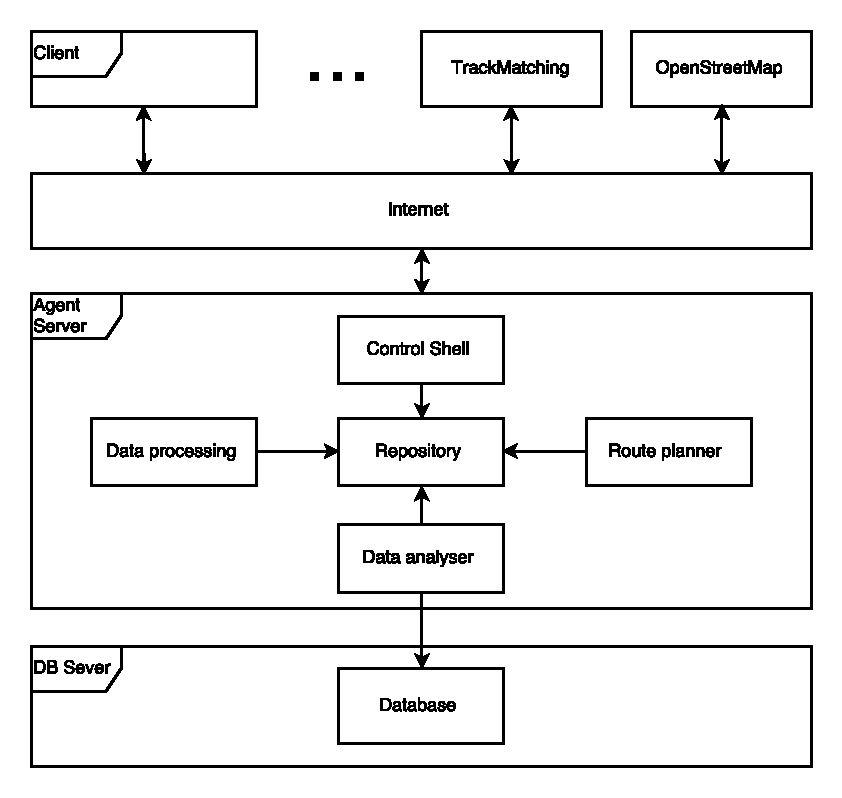
\includegraphics[width=1\textwidth]{figures/architecture.pdf}
    \caption{A course grained system overview.}
    \label{fig:systemoverview}
\end{figure}

The system has been designed as a combination of a client-server and a repository "blackboard" pattern. The main server module encapsulates most of the processing of the system. The clients represent the GPS-enabled devices that communicates live GPS data through an internet connection to the server, which in turn processes and analyses the data in different subsystems. The server architecture is designed as a repository structure, where the solution repository is the shared medium of the subsystems. This architecture is well-known within artificial intelligence, where the solution is gradually built from different contributing systems, which is why we have chosen this structure of the system. Initially, the solution repository contains nothing but the problem specification, which is the set of route requests from the clients. The job of the subsystems is to transform the specification into a solution. This is done gradually by invoking the different subsystems to perform operations on the problem specification until a partial solution can be sent back to the client(s). The control shell module controls which subsystem that should be invoked, based on the contents of the solution repository. \todo{Consider if we should give a concrete example? or describe more.}
\todo{Consider if we should divide the database onto another server --> changing the architecture to 2 servers.}
%The flowchart shows how the user inputs their destination at the start, which sent to a central server together with the source start address. Ther server then uses the data to calculate a route based on the request. The route calculation is based on a initial model of the roadnetwork, such as speedlimits and other restrictions on the roads, and also historical data that have been gathered over time from the users. The route is then sent back to the user, while driving the user will send data back about the drive, this will be the GPS points of the route. This information is then processed and analyzed to check if traffic conditions are as they are supposed to be, and if not the information can be used to recalculate routes for all the drivers which are passing through a that given segment.\todo{review section to describe new architecture}

\section{Client-server communcation}
As mentioned in the former section, we will be using a client-server structure. The reason behind this choice, is we need to be able to send information back and forth.
The client server interface is built upon the Java ServerSocket and the Java Socket, which handles opening a port, accepting a connection, and connecting to such a port, through a TCP connection.
The client sends a RequestID command to the server, where the server responds with sending back a ID to the client, the ID is a integer, which simply counts one up after each RequestID. 
%The client server interface handles connection to the server,
%sending acknowledgements of receiving the complete data,
%and the management of session IDs. \todo{Skal skrives færdig}

%How do we communicate between server and client? \todo{Skriv om hvordan vi har opbygget client-server arkitekturen.}
\section{Data Preprocessing}
The Beijing dataset consists timestamped samples of gps-coordinates. The format of the samples is (id, date time, longitude, latitude). However since GPS measurements can be inaccurate, it is not always possible to directly infer which road the sample was taken on. Consequently the coordinates must be map-matched to a road, such that positions on the road can be inferred. To perform map-matching, the system calls the TrackMatching webservice\cite{TrackMatching}. This service exposes an API for map-matching to the OpenStreetMap service and given a dataset of raw GPS-coordinates returns a map-matched dataset in JSON format. 
\todo{write about how and why map generation}
\todo{write about how and why we design DB and store data in SQL database}
\section{Data analysis}
\todo{How do we analyse the data? What information do we infer (speed, probability of traffic congestion, the design of the cost function to change based on traffic data? How are bayesian networks involved?}
There are 2 processes involved in keeping the data for the map realistic:
\begin{itemize}
	\item Traffic pattern analysis of historical data
	\item Live traffic data analysis
\end{itemize}

The main idea of the traffic pattern analysis is that the data gathered over a given period, at some point will be bulk processed to see if traffic patterns keep the same. Such that the system allways have the best image of the traffic for a particular day, and use these patterns for the best route calculation.

The live traffic data analysis is used check if there are any abnormalities at a given segment, and then being able to propagate this to devices that are going through that segment. Eventually redirecting drivers such that they don't end up at a congested segment, unless nothing else is possible.
\section{Route planning}
\todo{How do we plan the routes? A*/D*, heuristic and cost function for capacity of roads ....}
